\section{SIR-Modell für Deutschland}\label{sec:Resultate-SIR}
In \autoref{fig:SIR_Deutschland} sind die drei Kennzahlen des SIR-Modells für Deutschland in drei Graphen dargestellt.
\begin{figure}[H]
    \centering
    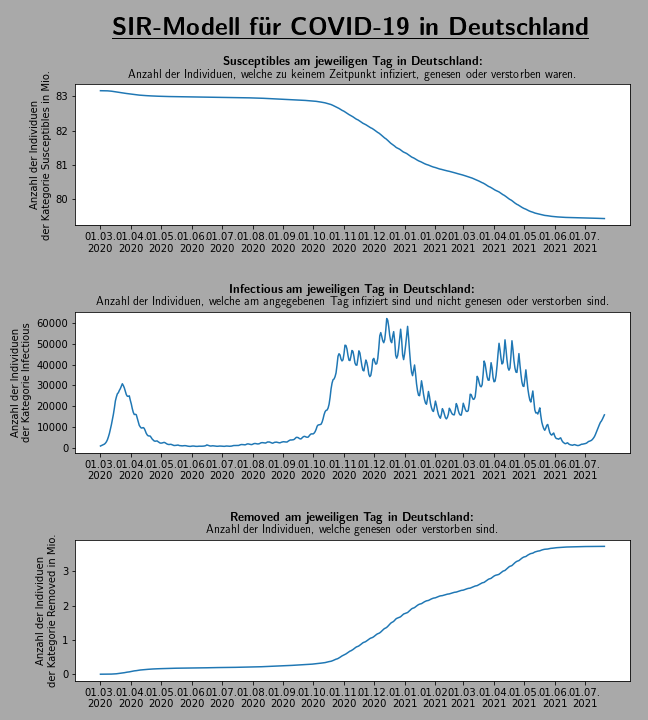
\includegraphics[width = 0.95\textwidth]{figures/Ergebnisse/SIR_Modell_Deutschland.png}
    \caption{Die drei Kennzahlen des SIR-Modells für Deutschland in drei Graphen.}
    \label{fig:SIR_Deutschland}
\end{figure}

Von den 3.748.038 gemeldeten Fällen weisen 46.033 Meldungen (1,2\%) Inkonsistenzen auf. Dies entspricht fast der maximalen Zahl der Menschen in Kategorie \glqq{}infectious\grqq{} von ca. 60.000.
In 37757 Fällen liegt das Meldedatum vor dem Referenzdatum, das heißt die Person ist nach der hier verwendeten Interpretation genesen bzw. gestorben bevor sie sich angesteckt hat. In 8276 Fällen liegt das Referenzdatum mehr als 30 Tage vor dem Referenzdatum, die Person ist also mehr als 30 Tage krank, was laut RKI sehr unwahrscheinlich ist.\autocite{RKI_Bulletin}

1409 Fälle wurden vor dem 01. März an das RKI gemeldet. Teilweise handelt es sich um authentische Meldungen, teilweise um fragwürdige Meldungen. Da die Gesamtzahl jedoch unter einem Prozent liegt, werden die Fälle in \autoref{fig:SIR_Deutschland} zum 01. März hinzugerechnet.